\newcommand{\coursemodule}{Module 05}
% ════════════════════════════════════════════════════════════════════════════
% Pixels, Frames & Transformers: shared Beamer preamble (WUR style)
% Adapted from the preamble of Bags, Vectors & Transformers.
%
% Use in a module deck (from <part>/<module>/slides/):
%   \newcommand{\coursemodule}{Module 01}
%   % ════════════════════════════════════════════════════════════════════════════
% Pixels, Frames & Transformers: shared Beamer preamble (WUR style)
% Adapted from the preamble of Bags, Vectors & Transformers.
%
% Use in a module deck (from <part>/<module>/slides/):
%   \newcommand{\coursemodule}{Module 01}
%   % ════════════════════════════════════════════════════════════════════════════
% Pixels, Frames & Transformers: shared Beamer preamble (WUR style)
% Adapted from the preamble of Bags, Vectors & Transformers.
%
% Use in a module deck (from <part>/<module>/slides/):
%   \newcommand{\coursemodule}{Module 01}
%   \input{../../../shared/preamble.tex}
%   \begin{document}
%   \moduletitle{Images as Data}
%   ...
% Compile with: latexmk -pdf <deck>.tex
% ════════════════════════════════════════════════════════════════════════════

\documentclass[aspectratio=169]{beamer}

% ── Packages ────────────────────────────────────────────────────────────────
\usepackage[T1]{fontenc}
\usepackage[utf8]{inputenc}
\usepackage{lmodern}
\usepackage{microtype}
\usepackage{xcolor}
\usepackage{tikz}
\usetikzlibrary{arrows.meta, positioning, calc, shapes.geometric, decorations.pathreplacing, matrix, fit}
\usepackage{booktabs}
\usepackage{fontawesome5}
\usepackage{array}
\usepackage[most]{tcolorbox}

\providecommand{\coursemodule}{}

% ── WUR color palette ───────────────────────────────────────────────────────
\definecolor{wurgreen}{HTML}{34B233}
\definecolor{darkgreen}{HTML}{1F6B1E}
\definecolor{lightgreen}{HTML}{E8F7E8}
\definecolor{darknavy}{HTML}{1A1A2E}
\definecolor{midgray}{HTML}{6B7280}
\definecolor{lightgray}{HTML}{F3F4F6}
\definecolor{bodytext}{HTML}{1F2937}
\definecolor{codegreen}{HTML}{9AE6B4}
\definecolor{warnred}{HTML}{FEE2E2}
\definecolor{warnborder}{HTML}{EF4444}

% ── Beamer theme ────────────────────────────────────────────────────────────
\usetheme{default}
\usecolortheme{default}
\usefonttheme{professionalfonts}
\setbeamertemplate{navigation symbols}{}
\setbeamertemplate{itemize items}{\textcolor{wurgreen}{\textbullet}}
\setbeamertemplate{itemize subitem}{\textcolor{midgray}{--}}
\setbeamertemplate{enumerate items}{\textcolor{wurgreen}{\textbf{\insertenumlabel.}}}
\setbeamercolor{frametitle}{fg=white, bg=darknavy}
\setbeamertemplate{frametitle}{%
  \begin{beamercolorbox}[wd=\paperwidth, ht=1.1cm, dp=0.2cm, leftskip=0.6cm]{frametitle}
    \usebeamerfont{frametitle}\insertframetitle
  \end{beamercolorbox}%
}
\setbeamerfont{frametitle}{size=\large, series=\bfseries}
\setbeamercolor{background canvas}{bg=white}
\setbeamercolor{normal text}{fg=bodytext}
\setbeamerfont{normal text}{size=\small}
\setbeamertemplate{footline}{%
  \begin{beamercolorbox}[wd=\paperwidth, ht=0.4cm, dp=0.15cm]{footline}%
    \hspace{0.5cm}%
    \textcolor{midgray}{\tiny Pixels, Frames \& Transformers · \coursemodule\ · Wageningen University \& Research}%
    \hfill%
    \textcolor{midgray}{\tiny \insertframenumber}%
    \hspace{0.4cm}%
  \end{beamercolorbox}%
}

% ── Boxes ───────────────────────────────────────────────────────────────────
\tcbset{wurbase/.style={arc=3pt, boxrule=0.6pt, left=7pt, right=7pt, top=5pt, bottom=5pt,
                        fontupper=\small, before skip=4pt, after skip=4pt}}
\newtcolorbox{greenbox}[1][]{wurbase, colback=lightgreen, colframe=wurgreen, #1}
\newtcolorbox{graybox}[1][]{wurbase, colback=lightgray, colframe=lightgray, #1}
\newtcolorbox{navybox}[1][]{wurbase, colback=darknavy, colframe=darknavy, colupper=white, #1}
\newtcolorbox{warnbox}[1][]{wurbase, colback=warnred, colframe=warnborder, #1}
\newtcolorbox{codebox}[1][]{wurbase, colback=darknavy, colframe=darknavy, colupper=white,
                            fontupper=\ttfamily\scriptsize, left=6pt, top=4pt, bottom=4pt, #1}

% ── Title slide ─────────────────────────────────────────────────────────────
\newcommand{\moduletitle}[1]{%
{
\setbeamertemplate{footline}{}
\begin{frame}[plain]
  \begin{tikzpicture}[remember picture, overlay]
    \fill[darknavy] (current page.south west) rectangle (current page.north east);
    \fill[wurgreen] (current page.south west) rectangle ([xshift=0.45cm]current page.north west);
    \node[anchor=west, text=white, font=\huge\bfseries, text width=13cm]
      at ([xshift=1.1cm, yshift=1.2cm]current page.west) {Pixels, Frames \& Transformers};
    \node[anchor=west, text=wurgreen, font=\large, text width=13cm]
      at ([xshift=1.1cm, yshift=0.05cm]current page.west) {#1 · \coursemodule};
    \node[anchor=west, text=midgray, font=\small, text width=12cm]
      at ([xshift=1.1cm, yshift=-1.5cm]current page.west)
      {Denise J. Roth, PhD Candidate\\
       Strategic Communication Group · Wageningen University \& Research};
  \end{tikzpicture}
\end{frame}
}}

% ── Small helpers ───────────────────────────────────────────────────────────
\newcommand{\keyterm}[1]{\textbf{\textcolor{darkgreen}{#1}}}
\newcommand{\muted}[1]{\textcolor{midgray}{#1}}
\newcommand{\credit}[1]{{\tiny\textcolor{midgray}{#1}}}
\newcommand{\notebookslide}[1]{%
\begin{frame}{In the Notebook}
\vspace{0.1cm}
#1
\end{frame}}
\newcommand{\nbitem}[2]{\item[\textcolor{wurgreen}{#1}] #2}

%   \begin{document}
%   \moduletitle{Images as Data}
%   ...
% Compile with: latexmk -pdf <deck>.tex
% ════════════════════════════════════════════════════════════════════════════

\documentclass[aspectratio=169]{beamer}

% ── Packages ────────────────────────────────────────────────────────────────
\usepackage[T1]{fontenc}
\usepackage[utf8]{inputenc}
\usepackage{lmodern}
\usepackage{microtype}
\usepackage{xcolor}
\usepackage{tikz}
\usetikzlibrary{arrows.meta, positioning, calc, shapes.geometric, decorations.pathreplacing, matrix, fit}
\usepackage{booktabs}
\usepackage{fontawesome5}
\usepackage{array}
\usepackage[most]{tcolorbox}

\providecommand{\coursemodule}{}

% ── WUR color palette ───────────────────────────────────────────────────────
\definecolor{wurgreen}{HTML}{34B233}
\definecolor{darkgreen}{HTML}{1F6B1E}
\definecolor{lightgreen}{HTML}{E8F7E8}
\definecolor{darknavy}{HTML}{1A1A2E}
\definecolor{midgray}{HTML}{6B7280}
\definecolor{lightgray}{HTML}{F3F4F6}
\definecolor{bodytext}{HTML}{1F2937}
\definecolor{codegreen}{HTML}{9AE6B4}
\definecolor{warnred}{HTML}{FEE2E2}
\definecolor{warnborder}{HTML}{EF4444}

% ── Beamer theme ────────────────────────────────────────────────────────────
\usetheme{default}
\usecolortheme{default}
\usefonttheme{professionalfonts}
\setbeamertemplate{navigation symbols}{}
\setbeamertemplate{itemize items}{\textcolor{wurgreen}{\textbullet}}
\setbeamertemplate{itemize subitem}{\textcolor{midgray}{--}}
\setbeamertemplate{enumerate items}{\textcolor{wurgreen}{\textbf{\insertenumlabel.}}}
\setbeamercolor{frametitle}{fg=white, bg=darknavy}
\setbeamertemplate{frametitle}{%
  \begin{beamercolorbox}[wd=\paperwidth, ht=1.1cm, dp=0.2cm, leftskip=0.6cm]{frametitle}
    \usebeamerfont{frametitle}\insertframetitle
  \end{beamercolorbox}%
}
\setbeamerfont{frametitle}{size=\large, series=\bfseries}
\setbeamercolor{background canvas}{bg=white}
\setbeamercolor{normal text}{fg=bodytext}
\setbeamerfont{normal text}{size=\small}
\setbeamertemplate{footline}{%
  \begin{beamercolorbox}[wd=\paperwidth, ht=0.4cm, dp=0.15cm]{footline}%
    \hspace{0.5cm}%
    \textcolor{midgray}{\tiny Pixels, Frames \& Transformers · \coursemodule\ · Wageningen University \& Research}%
    \hfill%
    \textcolor{midgray}{\tiny \insertframenumber}%
    \hspace{0.4cm}%
  \end{beamercolorbox}%
}

% ── Boxes ───────────────────────────────────────────────────────────────────
\tcbset{wurbase/.style={arc=3pt, boxrule=0.6pt, left=7pt, right=7pt, top=5pt, bottom=5pt,
                        fontupper=\small, before skip=4pt, after skip=4pt}}
\newtcolorbox{greenbox}[1][]{wurbase, colback=lightgreen, colframe=wurgreen, #1}
\newtcolorbox{graybox}[1][]{wurbase, colback=lightgray, colframe=lightgray, #1}
\newtcolorbox{navybox}[1][]{wurbase, colback=darknavy, colframe=darknavy, colupper=white, #1}
\newtcolorbox{warnbox}[1][]{wurbase, colback=warnred, colframe=warnborder, #1}
\newtcolorbox{codebox}[1][]{wurbase, colback=darknavy, colframe=darknavy, colupper=white,
                            fontupper=\ttfamily\scriptsize, left=6pt, top=4pt, bottom=4pt, #1}

% ── Title slide ─────────────────────────────────────────────────────────────
\newcommand{\moduletitle}[1]{%
{
\setbeamertemplate{footline}{}
\begin{frame}[plain]
  \begin{tikzpicture}[remember picture, overlay]
    \fill[darknavy] (current page.south west) rectangle (current page.north east);
    \fill[wurgreen] (current page.south west) rectangle ([xshift=0.45cm]current page.north west);
    \node[anchor=west, text=white, font=\huge\bfseries, text width=13cm]
      at ([xshift=1.1cm, yshift=1.2cm]current page.west) {Pixels, Frames \& Transformers};
    \node[anchor=west, text=wurgreen, font=\large, text width=13cm]
      at ([xshift=1.1cm, yshift=0.05cm]current page.west) {#1 · \coursemodule};
    \node[anchor=west, text=midgray, font=\small, text width=12cm]
      at ([xshift=1.1cm, yshift=-1.5cm]current page.west)
      {Denise J. Roth, PhD Candidate\\
       Strategic Communication Group · Wageningen University \& Research};
  \end{tikzpicture}
\end{frame}
}}

% ── Small helpers ───────────────────────────────────────────────────────────
\newcommand{\keyterm}[1]{\textbf{\textcolor{darkgreen}{#1}}}
\newcommand{\muted}[1]{\textcolor{midgray}{#1}}
\newcommand{\credit}[1]{{\tiny\textcolor{midgray}{#1}}}
\newcommand{\notebookslide}[1]{%
\begin{frame}{In the Notebook}
\vspace{0.1cm}
#1
\end{frame}}
\newcommand{\nbitem}[2]{\item[\textcolor{wurgreen}{#1}] #2}

%   \begin{document}
%   \moduletitle{Images as Data}
%   ...
% Compile with: latexmk -pdf <deck>.tex
% ════════════════════════════════════════════════════════════════════════════

\documentclass[aspectratio=169]{beamer}

% ── Packages ────────────────────────────────────────────────────────────────
\usepackage[T1]{fontenc}
\usepackage[utf8]{inputenc}
\usepackage{lmodern}
\usepackage{microtype}
\usepackage{xcolor}
\usepackage{tikz}
\usetikzlibrary{arrows.meta, positioning, calc, shapes.geometric, decorations.pathreplacing, matrix, fit}
\usepackage{booktabs}
\usepackage{fontawesome5}
\usepackage{array}
\usepackage[most]{tcolorbox}

\providecommand{\coursemodule}{}

% ── WUR color palette ───────────────────────────────────────────────────────
\definecolor{wurgreen}{HTML}{34B233}
\definecolor{darkgreen}{HTML}{1F6B1E}
\definecolor{lightgreen}{HTML}{E8F7E8}
\definecolor{darknavy}{HTML}{1A1A2E}
\definecolor{midgray}{HTML}{6B7280}
\definecolor{lightgray}{HTML}{F3F4F6}
\definecolor{bodytext}{HTML}{1F2937}
\definecolor{codegreen}{HTML}{9AE6B4}
\definecolor{warnred}{HTML}{FEE2E2}
\definecolor{warnborder}{HTML}{EF4444}

% ── Beamer theme ────────────────────────────────────────────────────────────
\usetheme{default}
\usecolortheme{default}
\usefonttheme{professionalfonts}
\setbeamertemplate{navigation symbols}{}
\setbeamertemplate{itemize items}{\textcolor{wurgreen}{\textbullet}}
\setbeamertemplate{itemize subitem}{\textcolor{midgray}{--}}
\setbeamertemplate{enumerate items}{\textcolor{wurgreen}{\textbf{\insertenumlabel.}}}
\setbeamercolor{frametitle}{fg=white, bg=darknavy}
\setbeamertemplate{frametitle}{%
  \begin{beamercolorbox}[wd=\paperwidth, ht=1.1cm, dp=0.2cm, leftskip=0.6cm]{frametitle}
    \usebeamerfont{frametitle}\insertframetitle
  \end{beamercolorbox}%
}
\setbeamerfont{frametitle}{size=\large, series=\bfseries}
\setbeamercolor{background canvas}{bg=white}
\setbeamercolor{normal text}{fg=bodytext}
\setbeamerfont{normal text}{size=\small}
\setbeamertemplate{footline}{%
  \begin{beamercolorbox}[wd=\paperwidth, ht=0.4cm, dp=0.15cm]{footline}%
    \hspace{0.5cm}%
    \textcolor{midgray}{\tiny Pixels, Frames \& Transformers · \coursemodule\ · Wageningen University \& Research}%
    \hfill%
    \textcolor{midgray}{\tiny \insertframenumber}%
    \hspace{0.4cm}%
  \end{beamercolorbox}%
}

% ── Boxes ───────────────────────────────────────────────────────────────────
\tcbset{wurbase/.style={arc=3pt, boxrule=0.6pt, left=7pt, right=7pt, top=5pt, bottom=5pt,
                        fontupper=\small, before skip=4pt, after skip=4pt}}
\newtcolorbox{greenbox}[1][]{wurbase, colback=lightgreen, colframe=wurgreen, #1}
\newtcolorbox{graybox}[1][]{wurbase, colback=lightgray, colframe=lightgray, #1}
\newtcolorbox{navybox}[1][]{wurbase, colback=darknavy, colframe=darknavy, colupper=white, #1}
\newtcolorbox{warnbox}[1][]{wurbase, colback=warnred, colframe=warnborder, #1}
\newtcolorbox{codebox}[1][]{wurbase, colback=darknavy, colframe=darknavy, colupper=white,
                            fontupper=\ttfamily\scriptsize, left=6pt, top=4pt, bottom=4pt, #1}

% ── Title slide ─────────────────────────────────────────────────────────────
\newcommand{\moduletitle}[1]{%
{
\setbeamertemplate{footline}{}
\begin{frame}[plain]
  \begin{tikzpicture}[remember picture, overlay]
    \fill[darknavy] (current page.south west) rectangle (current page.north east);
    \fill[wurgreen] (current page.south west) rectangle ([xshift=0.45cm]current page.north west);
    \node[anchor=west, text=white, font=\huge\bfseries, text width=13cm]
      at ([xshift=1.1cm, yshift=1.2cm]current page.west) {Pixels, Frames \& Transformers};
    \node[anchor=west, text=wurgreen, font=\large, text width=13cm]
      at ([xshift=1.1cm, yshift=0.05cm]current page.west) {#1 · \coursemodule};
    \node[anchor=west, text=midgray, font=\small, text width=12cm]
      at ([xshift=1.1cm, yshift=-1.5cm]current page.west)
      {Denise J. Roth, PhD Candidate\\
       Strategic Communication Group · Wageningen University \& Research};
  \end{tikzpicture}
\end{frame}
}}

% ── Small helpers ───────────────────────────────────────────────────────────
\newcommand{\keyterm}[1]{\textbf{\textcolor{darkgreen}{#1}}}
\newcommand{\muted}[1]{\textcolor{midgray}{#1}}
\newcommand{\credit}[1]{{\tiny\textcolor{midgray}{#1}}}
\newcommand{\notebookslide}[1]{%
\begin{frame}{In the Notebook}
\vspace{0.1cm}
#1
\end{frame}}
\newcommand{\nbitem}[2]{\item[\textcolor{wurgreen}{#1}] #2}


\begin{document}

\moduletitle{Convolutional Neural Networks for Images}

% ─────────────────────────────────────────────────────────────────────────────
\begin{frame}{From Designed Features to Learned Features}
\vspace{0.2cm}
\centering
\begin{tikzpicture}[
  b/.style={draw=midgray, fill=lightgray, rounded corners=3pt, font=\footnotesize, align=center,
            inner sep=5pt, text width=2.6cm, minimum height=0.95cm},
  g/.style={draw=wurgreen, fill=lightgreen, rounded corners=3pt, font=\footnotesize, align=center,
            inner sep=5pt, text width=2.6cm, minimum height=0.95cm},
  arr/.style={-{Stealth[length=2mm]}, thick, color=midgray},
  lab/.style={font=\footnotesize\bfseries, anchor=east, text width=2.2cm, align=right}]
\node[lab] at (-0.3, 0) {Part 1};
\node[b] (p1) at (1.5, 0) {pixels};
\node[b, right=0.6cm of p1] (f1) {features \textbf{you} designed: colorfulness, faces, \ldots};
\node[b, right=0.6cm of f1] (c1) {classifier};
\draw[arr] (p1) -- (f1); \draw[arr] (f1) -- (c1);
\node[lab] at (-0.3, -1.6) {A CNN};
\node[g] (p2) at (1.5, -1.6) {pixels};
\node[g, right=0.6cm of p2] (f2) {filters the network \textbf{learns} from labeled examples};
\node[g, right=0.6cm of f2] (c2) {classifier};
\draw[arr] (p2) -- (f2); \draw[arr] (f2) -- (c2);
\draw[decorate, decoration={brace, amplitude=5pt, mirror}, thick, color=wurgreen]
  ([yshift=-0.15cm]p2.south west) -- node[below=6pt, font=\footnotesize, color=darkgreen] {trained together, end to end} ([yshift=-0.15cm]c2.south east);
\end{tikzpicture}

\vspace{0.4cm}
\raggedright
\begin{columns}[T]
\begin{column}{0.48\textwidth}
\begin{greenbox}
\textbf{The promise:} features you would never think of designing, tuned to your task.
\end{greenbox}
\end{column}
\begin{column}{0.48\textwidth}
\begin{warnbox}
\textbf{The price:} the network has to learn every filter from examples, so it needs many
labeled images.
\end{warnbox}
\end{column}
\end{columns}
\end{frame}

% ─────────────────────────────────────────────────────────────────────────────
\begin{frame}{Convolution: A Filter Sliding over Pixels}
\centering
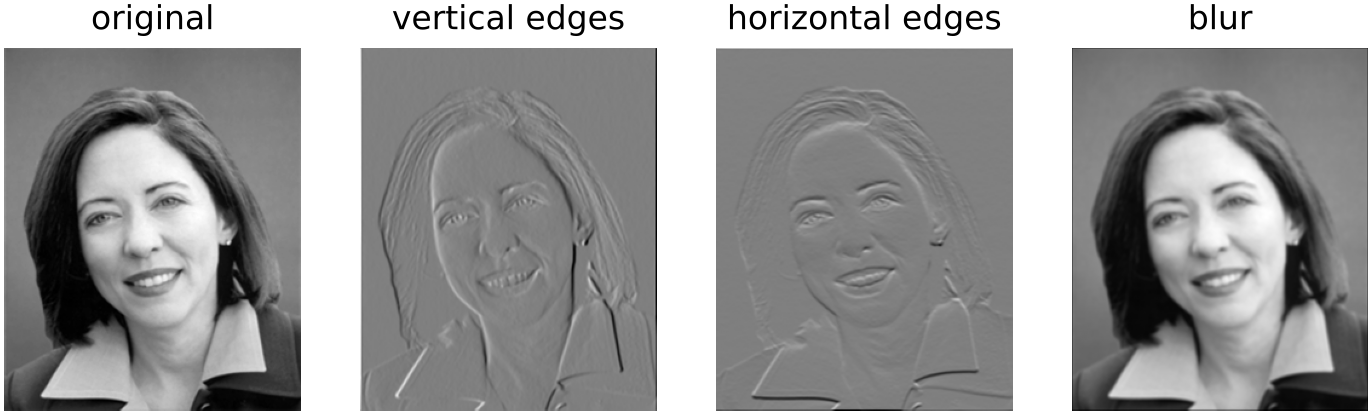
\includegraphics[width=0.8\textwidth]{figures/conv_filters.png}

\vspace{0.15cm}
\raggedright
\begin{columns}[c]
\begin{column}{0.27\textwidth}
\centering
{\footnotesize
$\begin{bmatrix} -1 & 0 & 1 \\ -2 & 0 & 2 \\ -1 & 0 & 1 \end{bmatrix}$\\[3pt]
\muted{the vertical-edge filter}}
\end{column}
\begin{column}{0.7\textwidth}
At every position the filter multiplies the pixels under it by its weights and adds them up.
The result, a \keyterm{feature map}, is bright wherever the image matches the pattern: here,
dark next to bright, from left to right. Weights that sum to 0 ignore overall brightness and
respond only to change.
\end{column}
\end{columns}
\vfill
\credit{Official portrait of Sen.\ Maria Cantwell, public domain, via unitedstates/images.}
\end{frame}

% ─────────────────────────────────────────────────────────────────────────────
\begin{frame}{Pooling, and Layers That Build on Each Other}
\begin{columns}[T]
\begin{column}{0.48\textwidth}
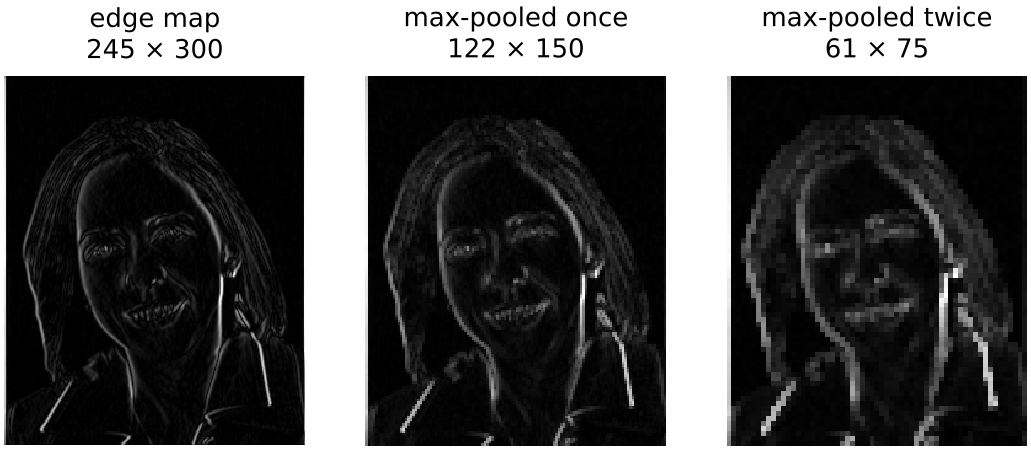
\includegraphics[width=\textwidth]{figures/pooling.png}

\vspace{0.1cm}
\keyterm{Max pooling} keeps the largest value of every 2 $\times$ 2 block: the map gets four times
smaller and a little less sensitive to exactly \emph{where} something is.
\end{column}
\begin{column}{0.49\textwidth}
\vspace{0.1cm}
\centering
\begin{tikzpicture}[
  s/.style={draw=wurgreen, fill=lightgreen, rounded corners=3pt, font=\footnotesize, align=center,
            inner sep=4pt, text width=3.6cm},
  arr/.style={-{Stealth[length=2mm]}, thick, color=midgray}]
\node[s] (a) {\textbf{early layers}\\ edges, color blobs};
\node[s, below=0.3cm of a] (b) {corners, textures};
\node[s, below=0.3cm of b] (c) {parts: eyes, wheels, letters};
\node[s, below=0.3cm of c] (d) {\textbf{later layers}\\ whole objects and scenes};
\draw[arr] (a) -- (b); \draw[arr] (b) -- (c); \draw[arr] (c) -- (d);
\end{tikzpicture}

\vspace{0.1cm}
\raggedright
\muted{Each layer combines the feature maps of the layer below. Nobody tells the network which
patterns to look for.}
\end{column}
\end{columns}
\end{frame}

% ─────────────────────────────────────────────────────────────────────────────
\begin{frame}{A Small CNN, Layer by Layer}
\vspace{0.3cm}
\centering
\begin{tikzpicture}[
  l/.style={draw=darknavy, fill=lightgray, rounded corners=2pt, font=\scriptsize, align=center,
            inner sep=2pt, text width=1.32cm, minimum height=1.3cm},
  o/.style={draw=darknavy, fill=darknavy, text=white, rounded corners=2pt, font=\scriptsize,
            align=center, inner sep=2pt, text width=1.32cm, minimum height=1.3cm},
  arr/.style={-{Stealth[length=1.6mm]}, thick, color=midgray}]
\node[l] (in) {image\\ $32 \times 32 \times 3$};
\node[l, right=0.2cm of in] (c1) {conv + ReLU\\ $32 \times 32 \times 32$};
\node[l, right=0.2cm of c1] (p1) {pool\\ $16 \times 16 \times 32$};
\node[l, right=0.2cm of p1] (c2) {conv + ReLU\\ $16 \times 16 \times 64$};
\node[l, right=0.2cm of c2] (p2) {pool\\ $8 \times 8 \times 64$};
\node[l, right=0.2cm of p2] (c3) {conv + ReLU\\ $8 \times 8 \times 128$};
\node[l, right=0.2cm of c3] (g) {global average pool\\ 128};
\node[o, right=0.2cm of g] (out) {linear\\ 10 classes};
\foreach \a/\b in {in/c1, c1/p1, p1/c2, c2/p2, p2/c3, c3/g, g/out} \draw[arr] (\a) -- (\b);
\end{tikzpicture}

\vspace{0.45cm}
\raggedright
\begin{columns}[T]
\begin{column}{0.48\textwidth}
\begin{itemize}
\item About \textbf{95,000 weights}, almost all in the convolution filters
\item Images get smaller (pooling) and ``deeper'' (more channels) as they pass through
\end{itemize}
\end{column}
\begin{column}{0.48\textwidth}
\begin{greenbox}
\keyterm{Global average pooling} reduces each feature map to one number, so the same network
accepts a 32 $\times$ 32 image and a 96 $\times$ 96 one.
\end{greenbox}
\end{column}
\end{columns}
\end{frame}

% ─────────────────────────────────────────────────────────────────────────────
\begin{frame}{Training in One Loop}
\begin{columns}[T]
\begin{column}{0.5\textwidth}
\begin{codebox}
for x, y in train\_loader:\hfill\textcolor{codegreen}{\# one batch}\\
\hspace*{1.5em}logits = model(x)\\
\hspace*{1.5em}loss = loss\_fn(logits, y)\\
\hspace*{1.5em}optimizer.zero\_grad()\\
\hspace*{1.5em}loss.backward()\hfill\textcolor{codegreen}{\# gradients}\\
\hspace*{1.5em}optimizer.step()\hfill\textcolor{codegreen}{\# nudge the weights}
\end{codebox}
\muted{One pass over all training images is an \textbf{epoch}. PyTorch computes every gradient
for you.}
\end{column}
\begin{column}{0.47\textwidth}
\begin{itemize}
\item \keyterm{Training set}: what the weights learn from
\item \keyterm{Validation set}: watched after every epoch to see when to stop
\item \keyterm{Test set}: used once, at the end, for an honest estimate
\end{itemize}
\vspace{0.1cm}
\begin{graybox}
On CIFAR-10 (50,000 labeled photos in ten classes), a network this small gets well beyond the
10\% of guessing in a few minutes on a GPU.
\end{graybox}
\end{column}
\end{columns}
\end{frame}

% ─────────────────────────────────────────────────────────────────────────────
\begin{frame}{Overfitting, and How to Fight It}
\begin{columns}[T]
\begin{column}{0.44\textwidth}
\centering
\begin{tikzpicture}[x=0.42cm, y=1.1cm]
\draw[-{Stealth[length=1.6mm]}, midgray] (0,0) -- (10.5,0) node[below left, font=\scriptsize] {epoch};
\draw[-{Stealth[length=1.6mm]}, midgray] (0,0) -- (0,3.2) node[above, font=\scriptsize] {loss};
\draw[very thick, wurgreen] plot[smooth] coordinates {(0.5,2.9) (2,1.8) (4,1.0) (6,0.55) (8,0.3) (10,0.15)};
\draw[very thick, darknavy] plot[smooth] coordinates {(0.5,3.0) (2,2.0) (3.5,1.55) (5,1.5) (7,1.8) (10,2.4)};
\draw[dashed, warnborder] (4.4,0) -- (4.4,2.9) node[above, font=\scriptsize, color=warnborder] {best epoch};
\node[font=\scriptsize, color=wurgreen, anchor=west] at (7.1,0.55) {training};
\node[font=\scriptsize, color=darknavy, anchor=west] at (7.0,2.75) {validation};
\end{tikzpicture}\\
\muted{\footnotesize schematic: the typical shape with too few images}
\end{column}
\begin{column}{0.53\textwidth}
With 1,000 images the network starts to \keyterm{memorize} them: training loss keeps falling,
validation loss turns around.
\begin{itemize}
\item \keyterm{Augmentation}: a slightly different version of each image every epoch (crops,
      flips). Only changes that keep the label true.
\item \keyterm{Dropout}: randomly switch off part of a layer during training
\item \keyterm{Early stopping}: keep the weights from the best validation epoch
\end{itemize}
\end{column}
\end{columns}

\begin{warnbox}
These help, but they stretch a small dataset; they don't replace a large one.
\end{warnbox}
\end{frame}

% ─────────────────────────────────────────────────────────────────────────────
\begin{frame}{Looking Inside the Network}
\begin{columns}[T]
\begin{column}{0.31\textwidth}
\begin{graybox}[height=2.6cm]
\raggedright\textbf{\faTh\ Filters}\\
Every learned weight can be shown. First-layer filters look like color blobs and edges.
\end{graybox}
\end{column}
\begin{column}{0.31\textwidth}
\begin{graybox}[height=2.6cm]
\raggedright\textbf{\faLayerGroup\ Activation maps}\\
What each filter responds to in one particular image.
\end{graybox}
\end{column}
\begin{column}{0.31\textwidth}
\begin{graybox}[height=2.6cm]
\raggedright\textbf{\faSearch\ Saliency maps}\\
The gradient of the class score with respect to each pixel: where a small change would matter
most.
\end{graybox}
\end{column}
\end{columns}

\vspace{0.15cm}
\begin{warnbox}
\textbf{Saliency maps are hints, not explanations.} Some popular methods give similar-looking maps
even for a network with random weights \muted{(Adebayo et al., 2018)}. To show that a model relies
on, say, the background, \textbf{test it}: replace the background and see whether the prediction
changes.
\end{warnbox}
\end{frame}

% ─────────────────────────────────────────────────────────────────────────────
\begin{frame}{Why Protest Photos Are Hard for a CNN from Scratch}
\begin{columns}[T]
\begin{column}{0.48\textwidth}
\begin{greenbox}
\textbf{\faTags\ Few labels}\\
CIFAR-10 has 50,000; we have a few hundred, a few dozen of them King's Day.
\end{greenbox}
\begin{greenbox}
\textbf{\faFolderOpen\ Noisy labels}\\
Commons categories say where an image was filed, not what it shows.
\end{greenbox}
\end{column}
\begin{column}{0.48\textwidth}
\begin{greenbox}
\textbf{\faUsers\ A class defined by people and signs}\\
in busy scenes, shrunk to 96 $\times$ 96 pixels, where signs become unreadable
\end{greenbox}
\begin{greenbox}
\textbf{\faImages\ Variety}\\
close-ups, crowds, aerial views; CIFAR-10 images are small and centered
\end{greenbox}
\end{column}
\end{columns}
\begin{navybox}
\textbf{Module 06:} borrow a network trained on millions of images, and learn only the last step
from your labels.
\end{navybox}
\end{frame}

% ─────────────────────────────────────────────────────────────────────────────
\notebookslide{
\begin{itemize}
\setlength{\itemsep}{5pt}
\nbitem{\faTh}{Filters and pooling by hand, on a portrait}
\nbitem{\faCubes}{A small CNN in PyTorch, trained on CIFAR-10}
\nbitem{\faChartLine}{Overfitting on 1,000 images, then augmentation, dropout and early stopping}
\nbitem{\faSearch}{Filters, activation maps and saliency maps, and their limits}
\nbitem{\faUsers}{The same network on protest photos, scored on your 40 coded images}
\nbitem{\faTrophy}{Your scoreboard: comparing with module 04}
\end{itemize}

\vspace{0.35cm}
\muted{\footnotesize part2\_vectors/05\_cnns\_for\_images/notebooks/05\_cnns\_for\_images\_exercises.ipynb
· 6 exercises · GPU recommended}
}

\end{document}
